% This document is for a tutorial video
%https://www.overleaf.com/learn/latex/LaTeX_video_tutorial_for_beginners_(video_1)

% All \ are Laytek commands

\documentclass[letterpaper,12pt]{article}  % Tells what type of document you want to make. Article is useful for scientific journal.
% https://www.youtube.com/watch?v=CxOCIfQhFmI&ab_channel=ShareLaTeX
% If you want a longer option you can use book or Journal class
% Can add chapters, split up documents into multiple files
\usepackage{tabularx} % extra features for tabular environment

\usepackage[utf8]{inputenc}  % lets you use accented UTF8 characters
\usepackage{amsmath}  % amsmath for more math options
\usepackage{graphicx}  % graphics package
\graphicspath{{Images/}}  % adds image path for putting in folder
% Bibtek is included automatically
%\usepackage[round]{natbib} % helps customize references
\usepackage[margin=1.25in,letterpaper]{geometry} % decreases margins
\usepackage{cite} % takes care of citations
\usepackage[final]{hyperref} % adds hyper links inside the generated PDF file
\hypersetup{
	colorlinks=true,       % false: boxed links; true: colored links
	linkcolor=blue,        % color of internal links
	citecolor=blue,        % color of links to bibliography
	filecolor=magenta,     % color of file links
	urlcolor=blue
}
\usepackage{blindtext}
\usepackage{fancyhdr}
\usepackage{enumitem}
\usepackage{sectsty}

\sectionfont{\fontsize{12}{12}\selectfont}

% \usepackage{natbib}  % Used for fancier biliography/citations
% \bibliographystyle{plainnat}  % the style setup
%\setlist{itemsep=1pt,leftmargin=*}

% Inserts key turns on and off text insert mode


%++++++++++++++++++++++++++++++++++++++++
% Decided not to do traditional title because it took to much space
% Using fancy header formatting https://www.overleaf.com/learn/latex/headers_and_footers#Standard_page_styles

\pagestyle{fancy}
\fancyhf{}
\rhead{CSE 701 -  Final Project - NPC Racer \newline Brendan Fallon}
\lhead{\today{}}  % April 14, 2021
\rfoot{Page \thepage}
\lfoot{}

\title{ % Make subtitle lines with \\
    NPC Racer \\
    \large A Performance Analysis of Game Agent Pathfinding
    Algorithms \\
    CAS 701 - Foundations of Modern Scientific Programming - \\
    Final Project}
\date{\today{}} %Wednesday, April 14, 2021
\author{Brendan Fallon}

%++++++++++++++++++++++++++++++++++++++++

% This is all preamble

\begin{document}  % Always need begin and end

\maketitle  % This makes the title of the document from the preamble

\tableofcontents  % makes a table of contents




\section{Implementation}
Implementation


1. Functional requirements, code requirements, and timeline ask for extensions.
2. Modules:
• char to bitmap parser
Going to have to make a character scanner parser to take in a 2D input
- looks like I can use the extraction operator: https://www.codeproject.com/Questions/210023/How-to-read-matrix-from-text-file-in-Cplusplus
%ifstream file;
%file.open( "C:\\TestFile.txt");
%int test[5] = {0};
%for( int i=0; i<5; i++)
%file >> test[i];
%file.close();
• AI prototype and derived pathfinding classes
• Maze class based or derived on Matrix but with bitmap or char type
• Timer/statistics module/helper static class for timing things.

- can split name spaces across multiple files:
% https://stackoverflow.com/questions/4093407/c-namespaces-and-defining-classes-in-separate-files
% e.g.
%// Canvas.h
%namespace TwoEngine
%{
%}
%
%// Primitive.h
%namespace TwoEngine
%{
%}




%\section{Future Work}






\addcontentsline{toc}{section}{References}  % adds a line to the table of contents, not done automatically
\bibliographystyle{plain}  % the style setup
%Enter the .bib style, can be plain or Plainnat with the nat package, can enter multiple filenames with coma
\bibliography{citations.bib}

\newpage
\appendix  % adding an appendix

%\section{Appendix: The files}
%\label{appendix:files}  % section for reference
%This is the Appendix

%\section{Appendix: Project evolution}
%\label{appendix:files}  % section for reference
%The project evolved over various stages and ideas based on limiting scope/complexity, time constraints, technology limitations, etc. I included a few screenshots on %how the modelling process evolved.

%\section{Appendix: GMF EVL Integration Tutorial}
%\label{appendix:tutorial}  % section for reference


\section{Appendix: Extending Generated Python Code Example}
\label{appendix:pythoncode}  % section for reference




\begin{figure}[h]  % h for here, p for separate page, b\t, or !
    \centering  % centers the figure in the page
    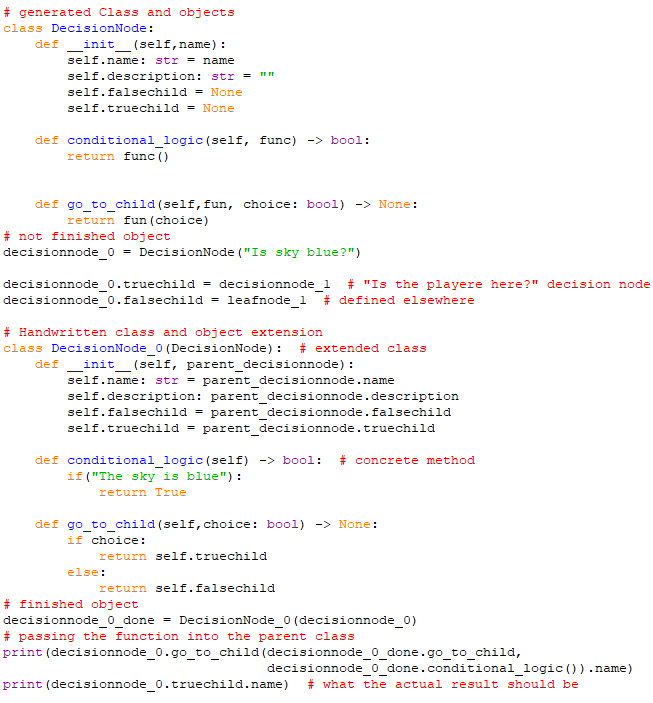
\includegraphics[width = 15 cm ]{Generated Code Extension Example.png}
    %\caption{Extending generated Python code using high-order functions.}
    \label{fig:code}
\end{figure}

%Using hand-written Python code to overwrite initialized generated code using high-order functions.



\end{document}

